\documentclass[a4paper]{article}

\usepackage[english]{babel}
\usepackage[utf8]{inputenc}
\usepackage{listings}
\usepackage{amsmath}

\usepackage{dcolumn}
\usepackage{booktabs}
\usepackage{tikz}
\usepackage{graphicx}

\usepackage{dcolumn}
\usepackage{booktabs}
\usepackage{tikz}
\usepackage{graphicx}

\usetikzlibrary{positioning,shapes,arrows}

\newcolumntype{M}[1]{D{.}{.}{1.#1}}

\title{Exercise Sheet 5}
\begin{document}
\maketitle

\section*{Problem 5.1}
1.)

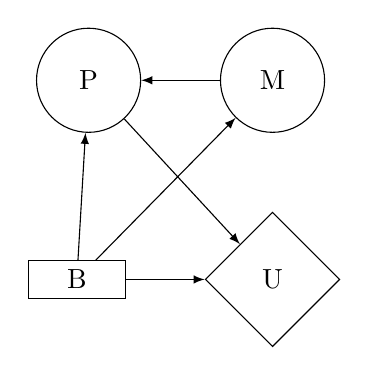
\begin{tikzpicture}[
  node distance=1cm and 1cm,
  mynode/.style={draw,circle,text width=1cm,align=center},
  mynodee/.style={draw,rectangle,text width=1cm,align=center},
  mynodeee/.style={draw,diamond,text width=1cm,align=center}
]

\node[mynode] (m) {M};
\node[mynode,left=of m] (p) {P};
\node[mynodeee,below=of m] (u) {U};
\node[mynodee,left=of u] (b) {B};

\path (p) edge[-latex] (u)
(b) edge[-latex] (p)
(m) edge[-latex] (p)
(b) edge[-latex] (m) 
(b) edge[-latex] (u);
\end{tikzpicture}

\noindent2.)

$B = 1$\\
$P(M) = 0,9$
\begin{align*}
    P(P) &= P(B,M) \cdot P(P|B,M) + P(B, \lnot M) \cdot P(P|B,\lnot M) + P(\lnot B, M) \cdot P(P|\lnot B, M) \\
    &+ P(\lnot B, \lnot M) \cdot P(P|\lnot B, \lnot M)\\
    &= 1\cdot 0.9\cdot 0.9 + 1\cdot 0.1 \cdot 0.5 + 0 \cdot 0.9 \cdot 0.8 + 0 \cdot 0.1 \cdot 0.3 = 0.86
\end{align*}
$EU(B) = 0.86 \cdot 2000 - 100 = 1620$
\\
\\

$B = 0$\\
$P(M) = 0,7$
\begin{align*}
    P(P) &= P(B,M) \cdot P(P|B,M) + P(B, \lnot M) \cdot P(P|B,\lnot M) + P(\lnot B, M) \cdot P(P|\lnot B, M) \\
    &+ P(\lnot B, \lnot M) \cdot P(P|\lnot B, \lnot M)\\
    &= 0\cdot 0.7\cdot 0.9 + 0\cdot 0.3 \cdot 0.5 + 1 \cdot 0.7 \cdot 0.8 + 1 \cdot 0.3 \cdot 0.3 = 0.65
\end{align*}
$EU(\lnot B) = 0.65 \cdot 2000 = 1300$

\newpage
\section*{Problem 5.2}
The monetary value itself is taken as utility here.\\
$A: [0.8, 4000; 0.2, 0]$\\
$B: [1, 3000; 0, 0]$\\
$C: [0.2, 4000; 0.8, 0]$\\
$D: [0.25, 3000; 0.75, 0]$\\
\\
$EU(A) = 0.8 * 4000 = 3200$\\ 
$EU(B) = 1.0 * 3000 = 3000$\\
$EU(C) = 0.2 * 4000 = 800$\\
$EU(D) = 0.25 * 3000 = 750$\\
\\
$B \prec A \Rightarrow  [p, B; (1-p), D] \prec [p, A; (1-p), D]$\\
\\
For this example, $p$ is set to $0.5$.\\
$U([p, B; (1-p), D]) = p\cdot 3000 + (1-p) 750 = 1500 + 375 = 1875$\\
$U([p, A; (1-p), D]) = p\cdot 3200 + (1-p) 750 = 1600 + 375 = 1975$\\
\\
$[p, B; (1-p), D] \prec [p, A; (1-p), D] \Leftrightarrow U([p, B; (1-p), D]) > U([p, A; (1-p), D])$\\
Aber: $U([p, B; (1-p), D]) < U([p, A; (1-p), D])$!\\
\textbf{Widerspruch.}\\
\end{document}
